\documentclass[11pt]{article}
\usepackage[T1]{fontenc}

\setlength{\topmargin}{-1.0cm} \setlength{\oddsidemargin}{-0.05in}
\setlength{\textheight} {8.5in} \setlength{\textwidth}{6.5in}
\setlength{\voffset}{-0.3in}
\renewcommand{\baselinestretch}{1.2}

\def\qed{\hspace*{\fill} \rule{2.5mm}{2.5mm} \\ }

\usepackage[dvips]{graphicx}
\usepackage[usenames]{color}
\usepackage{gastex}
\interdisplaylinepenalty=2500
\usepackage{fancyvrb}
\usepackage[Q=yes]{examplep}
\usepackage{float}
\usepackage{verbatim}
\usepackage{alltt}
\usepackage{fullpage}
\usepackage{url}
\usepackage{helvet}
\usepackage{bold-extra}
\usepackage{amssymb,amsmath}

\newcommand\vitem[1][]{\SaveVerb[%
    aftersave={\item[\textnormal{\UseVerb[#1]{vsave}}]}]{vsave}}

\title{\LARGE{\textbf{\fontfamily{\sfdefault}\selectfont Data Dealer Subscriber Agent Daily Report}}}
\author{Bj\"{o}rn Barrefors - bbarrefo@cse.unl.edu}

\date{\today}

\begin{document}

\maketitle

\section*{\textsc{Overview}}
Total amount of data subscribed: 2.04 TB

\section*{\textsc{Subscribed Datasets}}	
	\begin{description}
		\item \begin{alltt}/WJetsToLNu_HT-400ToInf_8TeV-madgraph_v2/Summer12_DR53X-PU_S10_START53_V7A-v1/AODSIM\end{alltt} \hfill \\
		\begin{tabular}{llll}
		Site & Rank & Size & \# Accesses \\ \hline
		\PVerb[pverb-verbatimfont=unchanged]{T2_US_Nebraska} & 600 & 1.96 TB & 10000 \\
		\end{tabular}

		\item \begin{alltt}/QCD_Pt-1400to1800_TuneZ2star_13TeV_pythia6/Spring14dr-PU20bx25_POSTLS170_V5-v1/AODSIM\end{alltt} \hfill \\
		\begin{tabular}{llll}
		Site & Rank & Size & \# Accesses \\ \hline
		\PVerb[pverb-verbatimfont=unchanged]{T2_RU_ITEP} & 500 & 0.08 TB & 1000 \\
		\end{tabular}
	\end{description}

\section*{\textsc{Top Five Datasets Not Subscribed}}
	\begin{description}
		\item \begin{alltt}/QCD_Pt-1800_TuneZ2star_13TeV_pythia6/Spring14dr-PU20bx25_POSTLS170_V5-v1/AODSIM\end{alltt} \hfill \\
		\begin{tabular}{llll}
		Rank & Size & \# Accesses \\ \hline
		150 & 0.04 TB & 100 \\
		\end{tabular}

		\item \begin{alltt} /TTH_HToBB_M-120_8TeV-pythia6/Summer12_DR53X-PU_S10_START53_V7A-v1/AODSIM\end{alltt} \hfill \\
		\begin{tabular}{llll}
		Rank & Size & \# Accesses \\ \hline
		100 & 0.43 TB & 90 \\
		\end{tabular}

		\item \begin{alltt} /TTH_HToBB_M-120_8TeV-pythia6/Summer12_DR53X-PU_S10_START53_V7A-v1/AODSIM\end{alltt} \hfill \\
		\begin{tabular}{llll}
		Rank & Size & \# Accesses \\ \hline
		100 & 0.43 TB & 90 \\
		\end{tabular}

		\item \begin{alltt} /TTH_HToBB_M-120_8TeV-pythia6/Summer12_DR53X-PU_S10_START53_V7A-v1/AODSIM\end{alltt} \hfill \\
		\begin{tabular}{llll}
		Rank & Size & \# Accesses \\ \hline
		100 & 0.43 TB & 90 \\
		\end{tabular}

		\item \begin{alltt} /TTH_HToBB_M-120_8TeV-pythia6/Summer12_DR53X-PU_S10_START53_V7A-v1/AODSIM\end{alltt} \hfill \\
		\begin{tabular}{llll}
		Rank & Size & \# Accesses \\ \hline
		100 & 0.43 TB & 90 \\
		\end{tabular}
	\end{description}

\section*{\textsc{Accesses For Above Datasets The Last Ten Days}}

	\begin{description}
		\item \begin{alltt}/WJetsToLNu_HT-400ToInf_8TeV-madgraph_v2/Summer12_DR53X-PU_S10_START53_V7A-v1/AODSIM\end{alltt}
		\begin{figure}[h]
			\begin{center}
			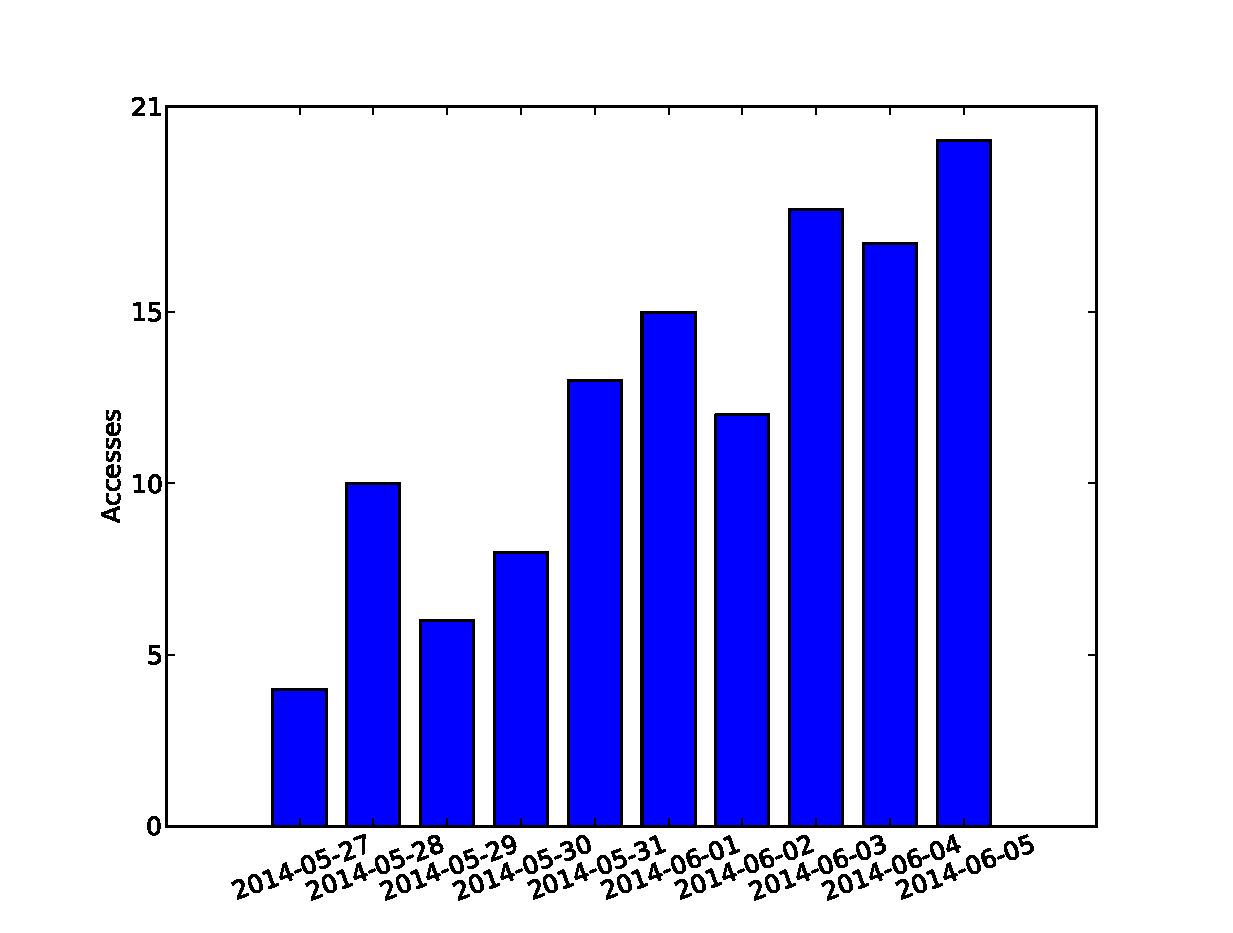
\includegraphics[scale=0.6]{d1.eps}
			\end{center}
		\end{figure}
	\end{description}

\end{document}
